\section{Data Geospasial}
Terdapat dua model data geospasial, yaitu model data raster dan model data vektor. 
Pada gambar \ref{datageospasial} dijelaskan tentang Klasifikasi model data geospasial.
\begin{figure}[ht]
	\centerline{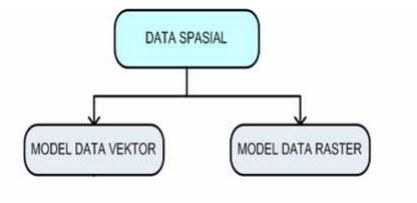
\includegraphics[width=1\textwidth]{figures/datageospasial.JPG}}
	\caption{Klasifikasi Model Data Geospasial.}
	\label{datageospasial}
	\end{figure}

\subsection{Data Vektor}
Model data vektor merupakan model data yang paling banyak digunakan.
Model ini berbasiskan pada titik dengan nilai koordinat (x,y) untuk membangun objek spasialnya. Objek yang dibangun terbagi menjadi tiga bagian lagi yaitu berupa titik (point), garis (line), dan area (polygon).

\subsubsection{Polygon}
Dalam artikel Mahendra menjelaskan Polygon merupakan representasi objek dalam dua dimensi. Contoh : danau,
persil tanah, dan lain-lain \cite{mahendra2014sistem}.
